

Om de dikte van het gate-oxide te bepalen is een simulatie in PSPICE niet voldoende. Het bepalen van de dikte vereist daarom een combinatie van simulaties en berekeningen die als volgt worden beschreven:
\begin{enumerate}
\item{\textbf{Totale gate capaciteit \emph{C\tss{G}} bepalen d.m.v. PSPICE simulatie}}
\\
Als eerst moet de totale gate capaciteit \emph{C\tss{G}} worden bepaald. Om deze \emph{C\tss{G}} te bepalen moeten we eerst de stroom \emph{I} bepalen door het oxide en de spanning \emph{V\tss{GS}} over het oxide bepalen. De formule die de relatie beschrijft tussen de stroom, spanning en de capaciteit \emph{C\tss{G}} is:
\begin{equation}
I = C_g(V\tss{GS}) \frac{dV\tss{GS}}{dt}
\end{equation}
Als we deze formule omschrijven naar
 \begin{equation}
 C_g(V\tss{GS})= \frac{I}{ \frac{dV\tss{GS}}{dt}}
 \end{equation}
kunnen we de \emph{C\tss{G}} bepalen. Deze simulatie dient een aantal keren te worden herhaald waarbij de \emph{W = 3.0$\mu$m} en de \emph{L} varieert tussen \emph{2.2$\mu$m} en \emph{4.8$\mu$m}. Dit geldt zowel voor de NMOS schakeling als voor de PMOS schakeling. Uit deze simulaties ontstaan grafieken die de \emph{C\tss{G}} bepalen voor verschillende waarden van de gate-source spanning V\tss{GS}. We zijn geïnteresseerd in de waarde van \emph{C\tss{G}} op het meest vlakke gedeelte van de grafiek. Deze waardes worden verder gebruikt bij stap 2.
\\
\\In figuur \ref{res:PMOS_schakeling} is de opstelling van de PMOS simulatie te zien en in figuur \ref{res:NMOS_schakeling} is de opstelling van NMOS schakeling te zien. In beide opstellingen is de weerstand \emph{R3 = 5k\textohm} en de stroom van de stroombron \emph{I2 = 1mA}. Verder zijn er ook twee probes aangesloten om de stroom en de spanning te meten. De simulatietijd is 100ps.

 \begin{figure} [h!]
 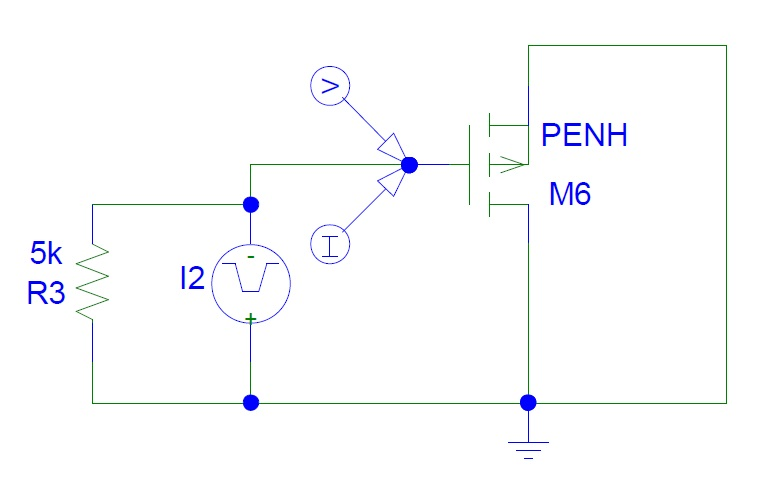
\includegraphics [scale = 0.7] {figures/PMOS}
 \caption{Opstelling voor bepalen van de \emph{C\tss{G}} van de PMOS transistor}
 \label{res:PMOS_schakeling}
 \end{figure}

 \begin{figure} [h!]
 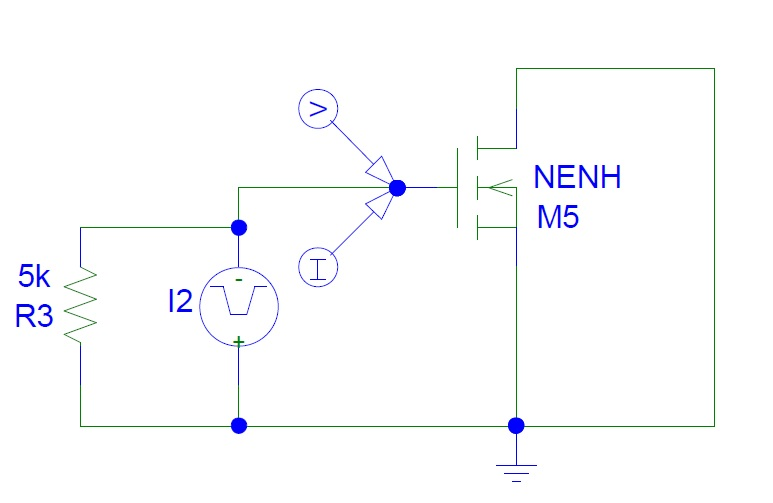
\includegraphics [scale = 0.7] {figures/NMOS}
 \caption{Opstelling voor bepalen van de \emph{C\tss{G}} van de NMOS transistor}
 \label{res:NMOS_schakeling}
 \end{figure}


\item{\textbf{Overlap capaciteit per lengte-eenheid \emph{C\tss{o}} bepalen m.b.v. MATLAB}}
\\
Als tweede stap gaan we de \emph{C\tss{o}} bepalen met behulp van de volgende formule:
\begin{equation}
C\tss{G} = W \ast C\tss{o} + L \ast W \ast C\tss{GC}
\end{equation}
Met behulp van MATLAB kunnen we de gevonden waarden van \emph{C\tss{G}} uit stap 1 met bijbehorende kanaallengtes \emph{L} invullen en zo een lineaire grafiek plotten. Als we deze grafiek doortrekken tot het punt waarbij \emph{L = 0}, kunnen we op de y-as de waarde uitlezen die gelijk is aan \emph{W \ast C\tss{o}}. Omdat \emph{W} vast staat kunnen we vervolgens \emph{C\tss{o}} bepalen.

\item{\textbf{Gate-channel capaciteit per oppervlakte-eenheid \emph{C\tss{GC}} berekenen}}
\\
Nadat de \emph{C\tss{G}} en de \emph{C\tss{o}} zijn bepaald kunnen we de \emph{C\tss{GC}} bepalen. Als we de formule uit stap 2 omschrijven krijgen we:
\begin{equation}
C\tss{GC} = \frac{C\tss{G} - C\tss{o} \ast W}{L \ast W}
\end{equation}
waaruit we \emph{C\tss{GC}} kunnen bepalen.


\item{\textbf{Dikte \emph{t\tss{ox}} van het gate oxide bepalen}}
\\
Als laatste stap kunnen we de dikte van het gate oxide bepalen aan de hand van de volgende formule:
\begin{equation}
t\tss{ox} = \frac{\epsilon\tss{ox}}{C\tss{GC}}
\end{equation}
Hierbij is \emph{$\epsilon$\tss{ox} = 35 fF/m}.



\end{enumerate}
